\section{Proof of Quantumness} \label{proof_of_quantumness}

\subsection{Interactive proof}
A proof serves as a means of persuading someone that a specific statement is true. We typically involve two parties when discussing proofs: \textit{a prover} and \textit{a verifier}. The prover aims to convince the verifier of the validity of a given statement, while the verifier's goal is to accept only accurate assertions. Before giving the definition of the interactive proof, we first recall that a language is simply a set of strings $L\subseteq \{0,1\}^*$. The definition of an interactive proof for a statement $x$ in a language $L$ is defined as follows:

\begin{defn}[Interactive proof]
    An interactive proof system for a language $L$ is a protocol between a computationally unrestricted prover $\mathcal{P}$ and a polynomial-time verifier $\mathcal{V}$ such that on input a statement $x$:
    \begin{itemize}
        \item \textbf{Completeness}: If $x\in L$, then an honest prover $\mathcal{P}$ that follows protocol should be able to convince the verifier $\mathcal{V}$ about the validity of the statement. 
        $$\forall x\in L, \Pr[(\mathcal{V}\leftrightarrow \mathcal{P})(x) \text{accepts }]=1.$$
        \item \textbf{Soundness $\epsilon$:} If $x \notin L$, then no malicious prover $\mathcal{P}'$ should be able to convince $\mathcal{V}$  with a success probability greater than $\epsilon$.
        $$\forall x\notin L, \forall \mathcal{P}', \Pr[(\mathcal{V}\leftrightarrow \mathcal{P}')(x) \text{accepts}]\leq \epsilon.$$
    \end{itemize}
\end{defn}
\begin{figure}[!htb]
	\centering
	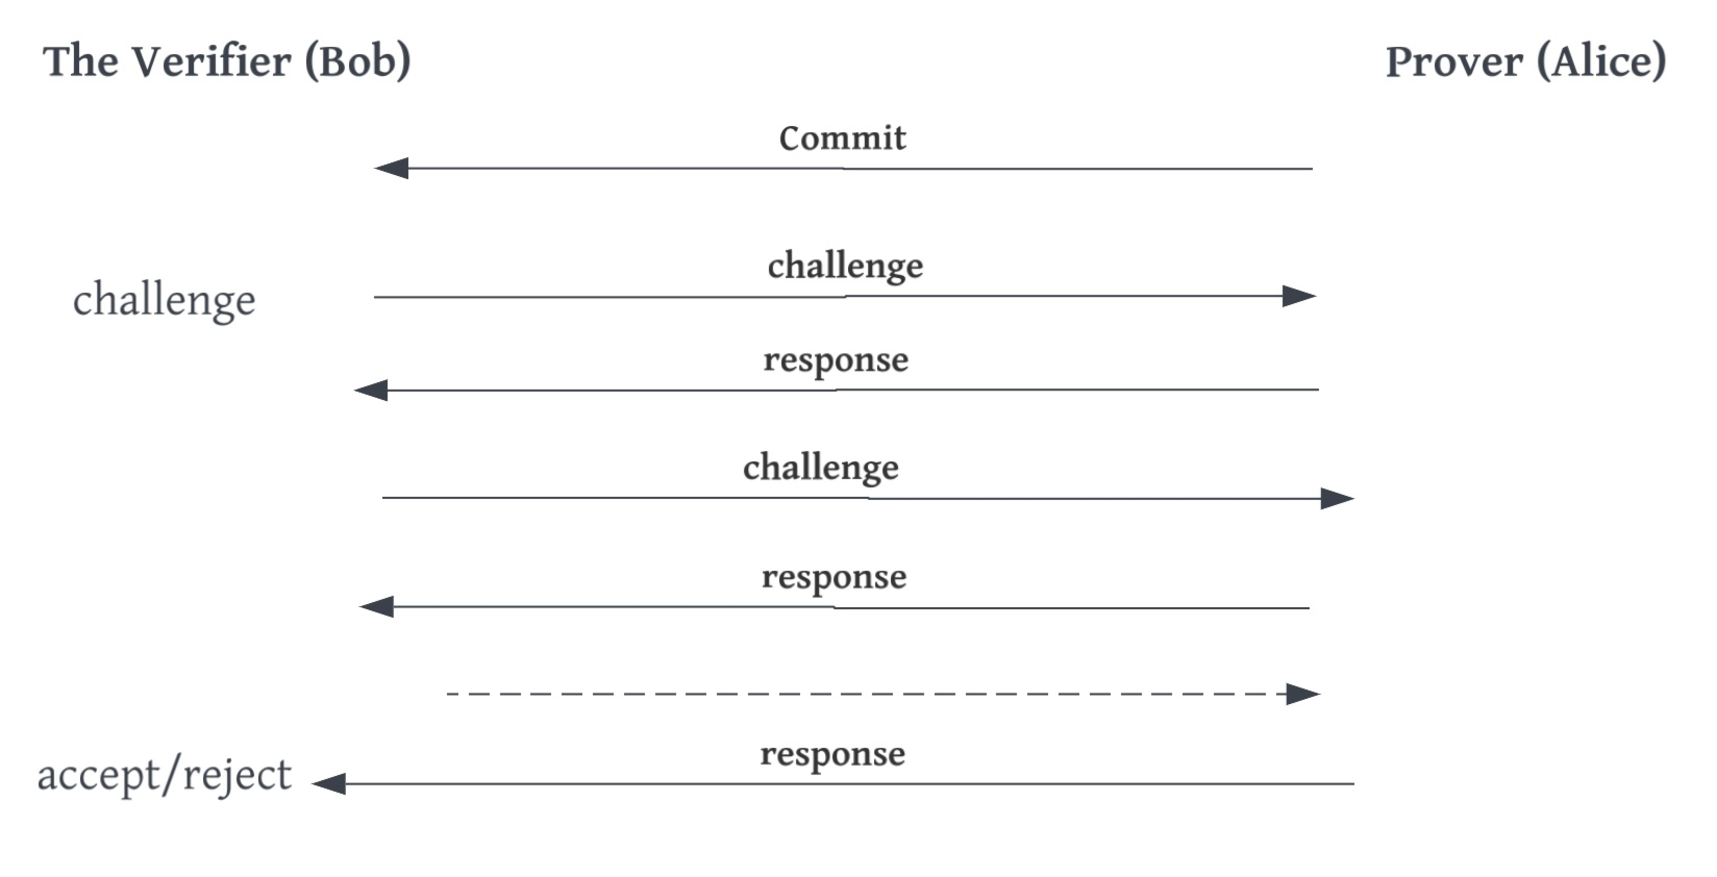
\includegraphics[scale = 0.35]{figures/IP.pdf}
	\caption{An interactive proof between a prover (Alice) and a verifier (Bob) typically has three main phases: commit, challenge, and response. The protocol may repeat the challenge-response phase multiple times to ensure the soundness property.}\label{fig:ip}
\end{figure}

\subsection{Proof of quantumness}
In recent years, under the efforts of building quantum computers, the verification of quantum behaviour has become significantly crucial. This underscores the necessity for a protocol in which a classical party can efficiently certify the quantum advantage of an untrusted device - the Proof of Quantumness. An interactive proof of quantumness~\cite{Brakerski18_Interactiveproofofquantumness,experiment_interactive_PoQ} is an interactive quantum verification protocol between two parties: a quantum prover $\mathcal{P}$ and a classical verifier $\mathcal{V}$. The verifier $\mathcal{V}$'s goal is to test the ``quantumness'' of the prover through an exchange of classical information. A common recent approach is to build the Interactive Proof of Quantumness protocol using TCFs.

%\begin{defn}[Proof of Quantumness~\cite{liu22poqdefn}]
%     A proof of quantumness is an interactive protocol with an efficient classical verifier satisfying:
%     \begin{itemize}
%         \item \textbf{Completeness.} There exists a polynomial-time quantum prover that can convince the verifier about its ``quantum'' ability.
%         \item \textbf{Soundness} $\epsilon$.
%          Any polynomial-time classical prover convinces the verifier with probability at most $\epsilon + \mathsf{negl}$ for some negligible function $\mathsf{negl}$.
%     \end{itemize}
%\end{defn}

\subsection{LWE}
The basic idea of employing the TFCs from LWE (Definition~\ref{defn:tcfsfromlwe}) to build the interactive proof of quantumness protocol is presented as follows:
\begin{enumerate}
    \item The verifier samples an LWE instance $\mathcal{I}=(\mathbf{A},\mathbf{y}=\mathbf{A}\mathbf{s}+\mathbf{e})$ together with a trapdoor $t_{k}=(\mathbf{s},\mathbf{e})$, and sends $\mathcal{I}$ and the description of the NTCFs $f_{\mathcal{I}}(\cdot)$ to the prover.
    \item The prover then:
    \begin{itemize}
        \item prepares a uniform superposition over $\mathbf{x}\in\{0,1\}^n$
        \begin{align}
            \frac{1}{\sqrt{2}^n}\sum_{\mathbf{x}\in\{0,1\}^n}\ket{\mathbf{x}},
        \end{align}
        \item evaluates $f_\mathcal{I}(\cdot)$ into an output register yields the state
        \begin{align}
            \sum_{\mathbf{x}\in\{0,1\}^n}\ket{\mathbf{x}}\ket{f_{\mathcal{I}}(\mathbf{x})},
        \end{align}        
        \item measures the output register to obtain $\mathbf{w}\in\mathcal{Y}$.
    The prover sends $\mathbf{w}$ to the verifier as the commitment for its quantum power.
    \end{itemize}
    \item The remaining state after measuring on the output register of the prover now is
    \begin{align}
        \frac{1}{\sqrt{2}}(\ket{\mathbf{x}_0}+\ket{\mathbf{x}_1})
    \end{align}
    where $\mathbf{x}_0$, $\mathbf{x}_1$ are two preimages of $\mathbf{w}$.
    \item The verifier challenge by asking the prover to measure on either the standard basis ($Z$ basis) $b=0$ or the Hadamard basis ($X$ basis) $b=1$.
    \item According to the verifier's challenge, the measurement outcome of the prover's state is:
    \begin{itemize}
        \item Standard basis: either $m=\mathbf{x}_0$ or $m=\mathbf{x}_1$, 
        \item Hadamard basis: $(c\in\{0,1\},m\in\{0,1\}^n)$ such that $m\cdot(\mathbf{x}_0+\mathbf{x}_1)=c$.
    \end{itemize}
    \item The verifier checks these tests: 
    \begin{itemize}
        \item Standard basis: simply check that $f_{\mathcal{I}}(m)=\mathbf{w}$.
        \item Hadamard basis: the verifier can recover $\mathbf{x}_0$, $\mathbf{x}_1$ from $\mathbf{y}$ using the trapdoor $t_k=(\mathbf{s},\mathbf{e})$, and check whether the pair $(m,c)$ satisfies $m\cdot(\mathbf{x}_0+\mathbf{x}_1)=c$.
    \end{itemize}

The protocol proceeds for $\lambda$ rounds. At the end of each round, the verifier samples a new problem instance and sends the new public key to the prover.
In a recent paper by Zhu~\cite{experiment_interactive_PoQ}, for each of the verifier’s possible choices, the experiment is repeated approximately $10^3$ times to collect statistics. 
\end{enumerate}

\begin{figure*}[!htp]
	\centering
	\begin{subfigure}[c]{\linewidth}
			\begin{quantikz}
\lstick{$f$} \setwiretype{c} & \gategroup[3,steps=7,style={rounded
    corners,fill=blue!10,draw=blue!50, inner
    xsep=5pt},background]{} & & & & \ctrl{0} & \setwiretype{n} & & & \lstick{$\mathsf{chall}$} & \setwiretype{c} \gategroup[3,steps=4,style={rounded
    corners,fill=blue!10,draw=blue!50, inner
    xsep=5pt},background]{} & & \ctrl{0} & \setwiretype{n} & \\
\setwiretype{n} & & \lstick{$\ket{\mathbf{0}}$} & \setwiretype{q} \qwbundle{n} & \gate{H^{\otimes n}} & \gate[2][5em]{U_f}\gateinput{$\mathbf{x}$}\gateoutput{$\mathbf{x}$}\wire[u]{c} & \qwbundle{n} & & & & & \qwbundle{n} & \gate{H^{\otimes n}}\wire[u]{c} & \meter{} & \setwiretype{c} \rstick{$\mathbf{m}$} & \setwiretype{n} & \\
\setwiretype{n} & & \lstick{$\ket{\mathbf{0}}$} & \setwiretype{q} \qwbundle{n-1} & & \gateinput{$\mathbf{y}$}\gateoutput{$\mathbf{y}\oplus f(x)$} & \qwbundle{n-1} & \meter{} & \setwiretype{c} \rstick{$\mathbf{w}$} & \setwiretype{n} & & & & & &
\end{quantikz}

			\caption{Two-round IPQ protocol, where $f$ is the TCF problem instance specified by the verifier. The prover executes the first round of the protocol, measuring the $\mathbf{y}$ register to obtain classical outcome $\mathbf{w}$. After receiving $\mathbf{w}$ from the prover the verifier communicates a random measurement basis $Z$ or $X$ for the prover to measure the $\mathbf{x}$ register in, yielding outcome $m\in\{0,1\}^n$. With knowledge of the problem instance's secret trapdoor, the verifier can efficiently verify the prover's response.}
	\end{subfigure}\label{fig:ipqlwe}
 \\
	\begin{subfigure}[c]{\linewidth}
		\begin{quantikz}
\lstick{$f$} \setwiretype{c} & \gategroup[3,steps=9,style={rounded
    corners,fill=blue!10,draw=blue!50, inner
    xsep=5pt},background]{} & & & & \ctrl{0} & \setwiretype{n} & & & & \\
\setwiretype{n} & & \lstick{$\ket{\mathbf{0}}$} & \setwiretype{q} \qwbundle{n} & \gate{H^{\otimes n}} & \gate[2][5em]{U_f}\gateinput{$x$}\gateoutput{$x$}\wire[u]{c} &\qwbundle{n} & \gate{U_h} & \gate{H^{\otimes n}} & \meter{} & \setwiretype{c} \rstick{$\mathbf{m}$} & \setwiretype{n} & \\
\setwiretype{n} & & \lstick{$\ket{\mathbf{0}}$} & \setwiretype{q} \qwbundle{n-1} & & \gateinput{$\mathbf{y}$}\gateoutput{$\mathbf{y}\oplus f(x)$} & \qwbundle{n-1} & \phantomgate{U_h} & \phantomgate{H^{\otimes n}} & \meter{} & \setwiretype{c} \rstick{$\mathbf{w}$} & \setwiretype{n} &
\end{quantikz}

		\caption{Single-round IPQ protocol, replacing the randomly chosen challenge $b$ specified by the verifier with a hash-function-based quantum random oracle.}
	\end{subfigure}\label{fig:ipqrlwe}
	\caption{\textbf{Quantum circuits for interactive proofs-of-quantumness (IPQ).} Blue boxes contain all quantum operations within the protocol with classical inputs and outputs.} \label{fig:IPQ_circuit.tex}
\end{figure*}

\noindent\textbf{Analysis.} For the proof of quantumness protocol, the post-quantum cryptography hardness assumption here is employed in a different way, where we do not require the prover to break something that the classical machine cannot. The protocol is constructed in a way that the security is preserved even against both \textit{classical} and \textit{quantum} prover. We use the \textit{rewinding} technique to distinguish between the classical and quantum cases. If a classical prover can cause the verifier to accept the statement, it can rewind and thus break the underlying hardness assumption which is computationally infeasible due to the hardness of the LWE problem. However, if the prover is ``quantum,'' it can persist with the verifier without breaking the underlying cryptographic assumption while performing measurements that cannot be reversed due to the no-cloning theorem.

Note the adaptive hardcore bit property plays an important role in this construction. Suppose there exists a prover capable of successfully navigating both verifier challenges. Specifically, given the problem instance $\mathcal{I}$, this prover can generate a tuple $(\mathbf{w}, b, \mathbf{x}_b, (m, c))$ with $b,c \in {0,1}$ that satisfies two checks with a probability significantly higher than $1/2$, i.e., $f_{\mathcal{I}}(\mathbf{x_b}) = \mathbf{w}$, $m \cdot (\mathbf{x}_0 \oplus \mathbf{x}_1) = c$, and $m \neq \mathbf{0}^n$.
It is important to note that in this scenario, the prover does not discover the entire claw $(\mathbf{x}_0, \mathbf{x}_1)$ but rather identifies one preimage $\mathbf{x}_b$ along with a linear function of the other preimage $\mathbf{x}_{1-b}$. Therefore, the \textbf{hardcore bit} property is indispensable, asserting that it is computationally challenging to find even a single bit of $\mathbf{x}_{1-b}$—meaning the prover cannot determine a single bit of $\mathbf{x}_{1-b}$, let alone the entire claw. 


\subsection{Non-interactive proof of quantumness from the RLWE problem}

Up till now, the hardcore bit property has only been shown for TCFs based on the LWE problem. However, it is still possible to construct a \textbf{non-interactive proof of quantumness} protocol based on other hardness assumptions. \cite{BrakerskiProofofQuantumness} employs the \textbf{random oracle heuristic} as a tool to reduce the round complexity of the proof of quantumness protocol which also makes it possible to implement the protocol in a single round and eliminates the need for the hard-core bit property. The quantum device must evaluate the random oracle on a quantum superposition.

Assume we have a hash function $h(\cdot)$. In the unitary model of quantum computing, consider this means that there exists a unitary $U_h$ that performs the mapping 
$$U_h: \ket{x}\ket{y} \mapsto \ket{x}\ket{y\oplus h(x)}$$
on the basis states.

For an element $x$, $\mathsf{BitDecomp}(x)$ is the binary representation of $x$. The proof of quantumness protocol is now parameterised by a hash function $h:\{0,1\}^n\to\{0,1\}$ as follows:
\begin{enumerate}
    \item The verifier generates the pair of public key and trapdoor $(k,t_k)$ and sends $k$ to the prover.
    \item The prover sends $\lambda$ tuple $\{(y_i,c_i,m_i)\}_{i\in[\lambda]}$, where $\lambda$ is the security parameter. The verifier initialises $\mathsf{count}=0$ and performs the following checks:
    \begin{itemize}
        \item It checks that all value $\{y_i\}_{i\in[\lambda]}$ are distinct.
        \item It uses the trapdoor to compute $x_{i,b}$ for each $i\in[\lambda]$ and $b\in\{0,1\}$. The verifier then checks $c_i=d_i^T\cdot(\mathsf{BitDecomp}(x_{i,0})+\mathsf{BitDecomp}(x_{i,1}))+h(x_{i,0})+h(x_{i,1})$. If $(c_i,d_i)$ satisfies this equation, it increases the value of $\mathsf{count}$ by $1$.
    \end{itemize}
    \item If $\mathsf{count}>0.75\lambda$, the verifier accepts, else it rejects.
\end{enumerate}

The second figure in~\ref{fig:IPQ_circuit.tex} represents the non-interactive proof of quantumness, which removes the interaction between the prover and the verifier during the challenge phase using the hash function $h(\cdot)$, as demonstrated above. Using the RLWE problem, we can significantly reduce the size of keys and the commitment of the construction.  


\textbf{Why can using the hash function can replace the hardcore bit property?} Recall that in the LWE-based proof of quantumness construction~\cite{Brakerski18_Interactiveproofofquantumness}, the prover applies the trapdoor claw-free function $f_{\mathcal{I}}$ on a uniform superposition of inputs and then measures the image register. It then obtains the value $w$, which will be sent to the verifier. The prover now has a state that is a superposition over $x_0$ and $x_1$. The prover then has to measure this state according to the challenge of the verifier: measure using the standard basis or Hadamard basis. A malicious prover that can break the protocol must be able to answer both challenges by the verifier simultaneously, which violates the \textit{hardcore bit property} and the hardness assumption. Using a one-bit hash function $h:\{0,1\}^n\to \{0,1\}$,~\cite{BrakerskiProofofQuantumness} generates the superposition over $(0,x_0,H(0,x_0))$ and $(1,x_1,H(1,x_1))$. The prover is then asked to measure the resulting state on a Hadamard basis only and send the outcome to the verifier, including a bit $c$ and the measurement outcome $m$. It holds that $(c,m)$ satisfies the hardcore predicate $c=m\cdot(x_0\oplus x_1)\oplus h(0,x_0)\oplus h(1,x_1)$. The verifier employs the trapdoor to recover $y,x_0,x_1$ and verifies whether the above equation is satisfied. The security of the protocol is upheld because an adversary cannot query the random oracle for both $(0,x_0)$ and $(1,x_1)$; thus, at least one value $h(0,x_0)$ or $h(1,x_1)$ remains random. This implies the malicious prover cannot compute $(c,d)$ satisfying the equation with a probability greater than $1/2$. Consequently, this also eliminates the need for the hardcore bit property.

\section{Experimental results}

This section gives the connection between result measurements in the original and experimental papers.

\begin{table*}[!htp]
    \centering
    \begin{tabular}{|c|c|c|c|c|c|c|c|}
    \hline
    \multirow{3}{*}{} &
    \multirow{3}{*}{\begin{tabular}[c]{@{}c@{}}Problem\end{tabular}} &  
    \multirow{3}{*}{\begin{tabular}[c]{@{}c@{}}Adaptive \\hardcore\\ bit \end{tabular}} &
    \multirow{3}{*}{\begin{tabular}[c]{@{}c@{}}IPOQ \end{tabular}} &
    \multirow{3}{*}{\begin{tabular}[c]{@{}c@{}}Random\\oracle
    \end{tabular}} &
    \multirow{3}{*}{\begin{tabular}[c]{@{}c@{}}Gate\\count \end{tabular}}&
    \multirow{3}{*}{\begin{tabular}[c]{@{}c@{}}Adversary\\type \end{tabular}}
    \\
    &   &   &  & & &\\
    &   &   &  & & &\\
    \hline
    \multirow{2}{*}{\cite{Brakerski18_Interactiveproofofquantumness}} &
    \multirow{2}{*}{\begin{tabular}[c]{@{}c@{}}LWE\end{tabular}} &  
    \multirow{2}{*}{\begin{tabular}[c]{@{}c@{}}\cmark \end{tabular}} &
    \multirow{2}{*}{\begin{tabular}[c]{@{}c@{}}\cmark  \end{tabular}} &
    \multirow{2}{*}{\begin{tabular}[c]{@{}c@{}}\xmark \end{tabular}} &
    \multirow{2}{*}{\begin{tabular}[c]{@{}c@{}}$n^2\log^2n$ \end{tabular}} &
    \multirow{2}{*}{\begin{tabular}[c]{@{}c@{}}classical\end{tabular}}
    \\
    &   &   &  & & &\\
    \hline
    
    \multirow{2}{*}{\cite{experiment_interactive_PoQ}} &
    \multirow{2}{*}{\begin{tabular}[c]{@{}c@{}}LWE\end{tabular}} &  
    \multirow{2}{*}{\begin{tabular}[c]{@{}c@{}}\cmark \end{tabular}} &
    \multirow{2}{*}{\begin{tabular}[c]{@{}c@{}}\cmark \end{tabular}} &
    \multirow{2}{*}{\begin{tabular}[c]{@{}c@{}}\xmark \end{tabular}} &
    \multirow{2}{*}{\begin{tabular}[c]{@{}c@{}}$n^2\log^2n$ \end{tabular}} &
    \multirow{2}{*}{\begin{tabular}[c]{@{}c@{}} classical
    \end{tabular}}
    \\
    &   &   &  & & &\\
    \hline
    \multirow{2}{*}{\cite{BrakerskiProofofQuantumness}} &
    \multirow{2}{*}{\begin{tabular}[c]{@{}c@{}}RLWE\end{tabular}} &  
    \multirow{2}{*}{\begin{tabular}[c]{@{}c@{}}\xmark \end{tabular}} &
    \multirow{2}{*}{\begin{tabular}[c]{@{}c@{}}\xmark \end{tabular}} &
    \multirow{2}{*}{\begin{tabular}[c]{@{}c@{}}\cmark  \end{tabular}} &
    \multirow{2}{*}{\begin{tabular}[c]{@{}c@{}}$n\log^2n$  \end{tabular}} &
    \multirow{2}{*}{\begin{tabular}[c]{@{}c@{}} quantum
    \end{tabular}}
    
    \\
    &   &   &  & & &\\
    \hline
    
    \multirow{2}{*}{\cite{experiment_non_interactive_PoQ}} &
    \multirow{2}{*}{\begin{tabular}[c]{@{}c@{}}LWE\end{tabular}} &  
    \multirow{2}{*}{\begin{tabular}[c]{@{}c@{}}\xmark \end{tabular}} &
    \multirow{2}{*}{\begin{tabular}[c]{@{}c@{}}\xmark \end{tabular}} &
    \multirow{2}{*}{\begin{tabular}[c]{@{}c@{}}\cmark \end{tabular}} &
    \multirow{2}{*}{\begin{tabular}[c]{@{}c@{}}$n^2\log^2n$  \end{tabular}} &
    \multirow{2}{*}{\begin{tabular}[c]{@{}c@{}} quantum
    \end{tabular}}
    
    \\
    &   &   &  & & &\\
    \hline
    \end{tabular}
    \label{t_2}
    \label{tab:compare}
    \caption{Comparison between the Proof of Quantumness protocols}
\end{table*}